
\section{Refining our Search}
At this point we have our initial ellipsoid \(E_0 = \ball(R, 0)\) defined in the
previous section, and we would like to fill out the body of the while loop. This
entails transforming \(E_k\) to some other ellipsoid \(E_{k+1}\) along with a
guarantee of some progress being made towards a final solution. In this section
we show how to produce \(E_{k+1}\) from \(E_k\), and in the following section we
argue that this yields a terminating algorithm.\\

\begin{figure}[h]
  \centering
  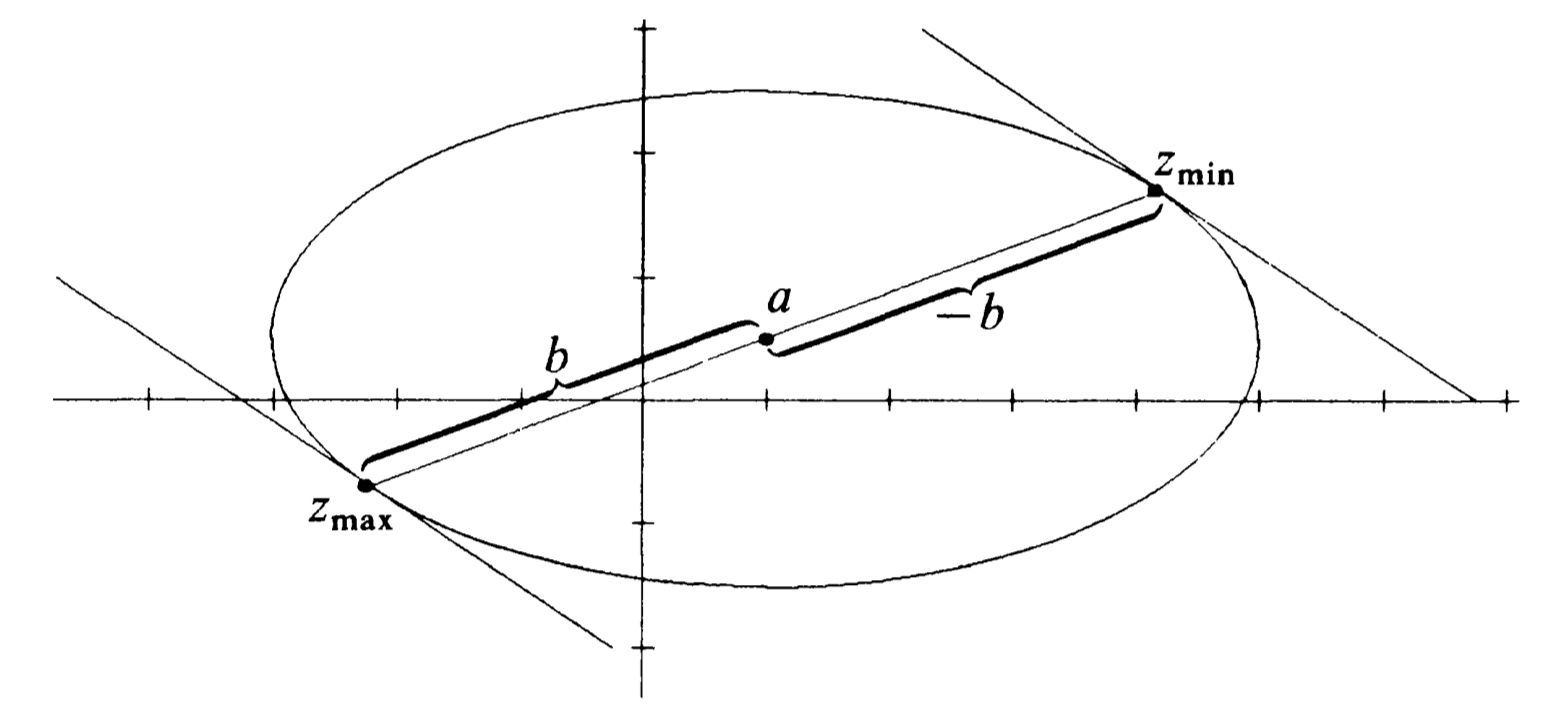
\includegraphics[width=0.9\textwidth]{img/ellipsoid-opt}
  \caption{Optimizing a cost function \(c\) over an ellipsoid}
  \label{fig:ellipsoid-opt}
\end{figure}
Suppose we have \(E_k = E(A_k, a_k)\). The first question we ask is:
\textit{``is \(a_k \in P\)?''}. This can be answered by testing \(a_k\) against
each linear inequality in \(Cx \leq d\). If \(c_i^t a_k \leq \gamma_i\) for each
\(i \in 1 \ldots m\) then \(a_k\) is in \(P\) and we may return \(a_k\) as a
witness of \(P\)'s non-emptiness. Otherwise, during some comparison we found an
inequality \(c^tx \leq \gamma\) that was violated by \(a_k\). We will use this
to perform an ellipsoidal cut, and from there we will construct a new
minimally-volumed ellipsoid containing the resulting convex body.\\


\subsection{Ellipsoidal Cuts}
Suppose we found inequality \(c^Tx \leq \gamma\) that is violated by center
\(a_k\). By convexity the hyperplane parallel to \(c\) through the center \(a\),
namely \(\{x \in \R^n : c^T x = c^T a\}\), does not intersect \(P\), and by
cutting \(E_k\) in half we have confined \(P\) to half of \(E_k\):
%
\begin{equation}\label{eq:ellipsoid-cut}
  E'(A_k, a_k, c) = E_k \cap \{ x \in \R^n : c^T x \leq c^T a_k\}.
\end{equation}

There are other cuts that we could have taken, but this one has the advantage of
making other parts of our algorithm simpler.\\

We take a brief detour to derive a quantity that will be used later. We start
with a question: how would one maximize a non-zero cost function \(c\) over
ellipsoid \(E(A,a)\)? This is tricky, but we do know how to maximize over a unit
ball \(\ball(1, a')\): the maximum value is found at vector \(a' +
\frac{c}{\norm{c}}\). We define \(Q := A^{1/2}\), and recall that \(Q^{-1}E(A,a)
= \ball(1, Q^{-1}a)\) (which was left as a homework exercise). Then we compute
as follows:
\begin{align*}
  \max\{c^T x | x \in E(A,a)\} &= \max\{c^T Q Q^{-1} x | Q^{-1}x \in Q^{-1} E(A,a)\}\\
    &= \max\{c^T Q y | y \in \ball(1, Q^{-1}a)\}\\
    &= c^T Q\left(Q^{-1}a + \frac{Qc}{\norm{Qc}}\right)\\
    &= c^T\Big(a + \underbrace{\frac{Ac}{\sqrt{c^TAc}}}_b\Big)
\end{align*}

Recalling that \(c^T\) is our cost function and \(a\) is the center of the
ellipse we conclude that \(b := Ac / \sqrt{c^T A c}\) is the vector between
\(a\) and the point on the boundary of \(E\) where \(c\) takes its maximal
value; this is illustrated in Figure~\ref{fig:ellipsoid-opt}, where the tangent
lines are parallel to the cost function \(c\).  Label \(z_{max}\) as the vector
in \(E\) where \(c\) takes its maximal value, and label \(z_{min}\) as the
vector in \(E\) where \(c\) takes its minimal value. It is clear that
\[z_{max} = a + b\]
\[z_{min} = a - b\]
This vector \(b\) turns
out to be important for a later computation.

%%%%%%%%%%%%%%%%%%%%%%%%%%%%%%%%%%%%%%%%%%%%%%%%%%%%%%%%%%%%%%%%%%%%%%%%%%%%%%%%
%%                           LOWNER JOHN ELLIPSOIDS                           %%
%%%%%%%%%%%%%%%%%%%%%%%%%%%%%%%%%%%%%%%%%%%%%%%%%%%%%%%%%%%%%%%%%%%%%%%%%%%%%%%%
\subsection{L\"owner John Ellipsoids}
Unfortunately, dividing ellipsoid \(E\) in half in (\ref{eq:ellipsoid-cut})
doesn't yield a new ellipsoid, so we don't yet have a new subproblem. Instead,
we would like to find a new ellipsoid that is smaller than the first that
contains the half ellipsoid \(E'\) (and therefore contains \(P\)).  To this end
we appeal to the following theorem, which is offered without proof.

\begin{theorem} \label{thm:lje}
  For every \(K \subseteq \R^n\) there exists a unique ellipsoid \(E\) of
  minimal volume containing \(K\).
\end{theorem}


\begin{defbox}
\begin{definition}[L\"owner John Ellipsoid]
    The \textbf{L\"owner John} ellipsoid of a convex body \(K\) is the smallest
    ellipsoid that contains \(K\), as given by Theorem~\ref{thm:lje}.
\end{definition}

\end{defbox}

\begin{figure}[h]
  \centering
  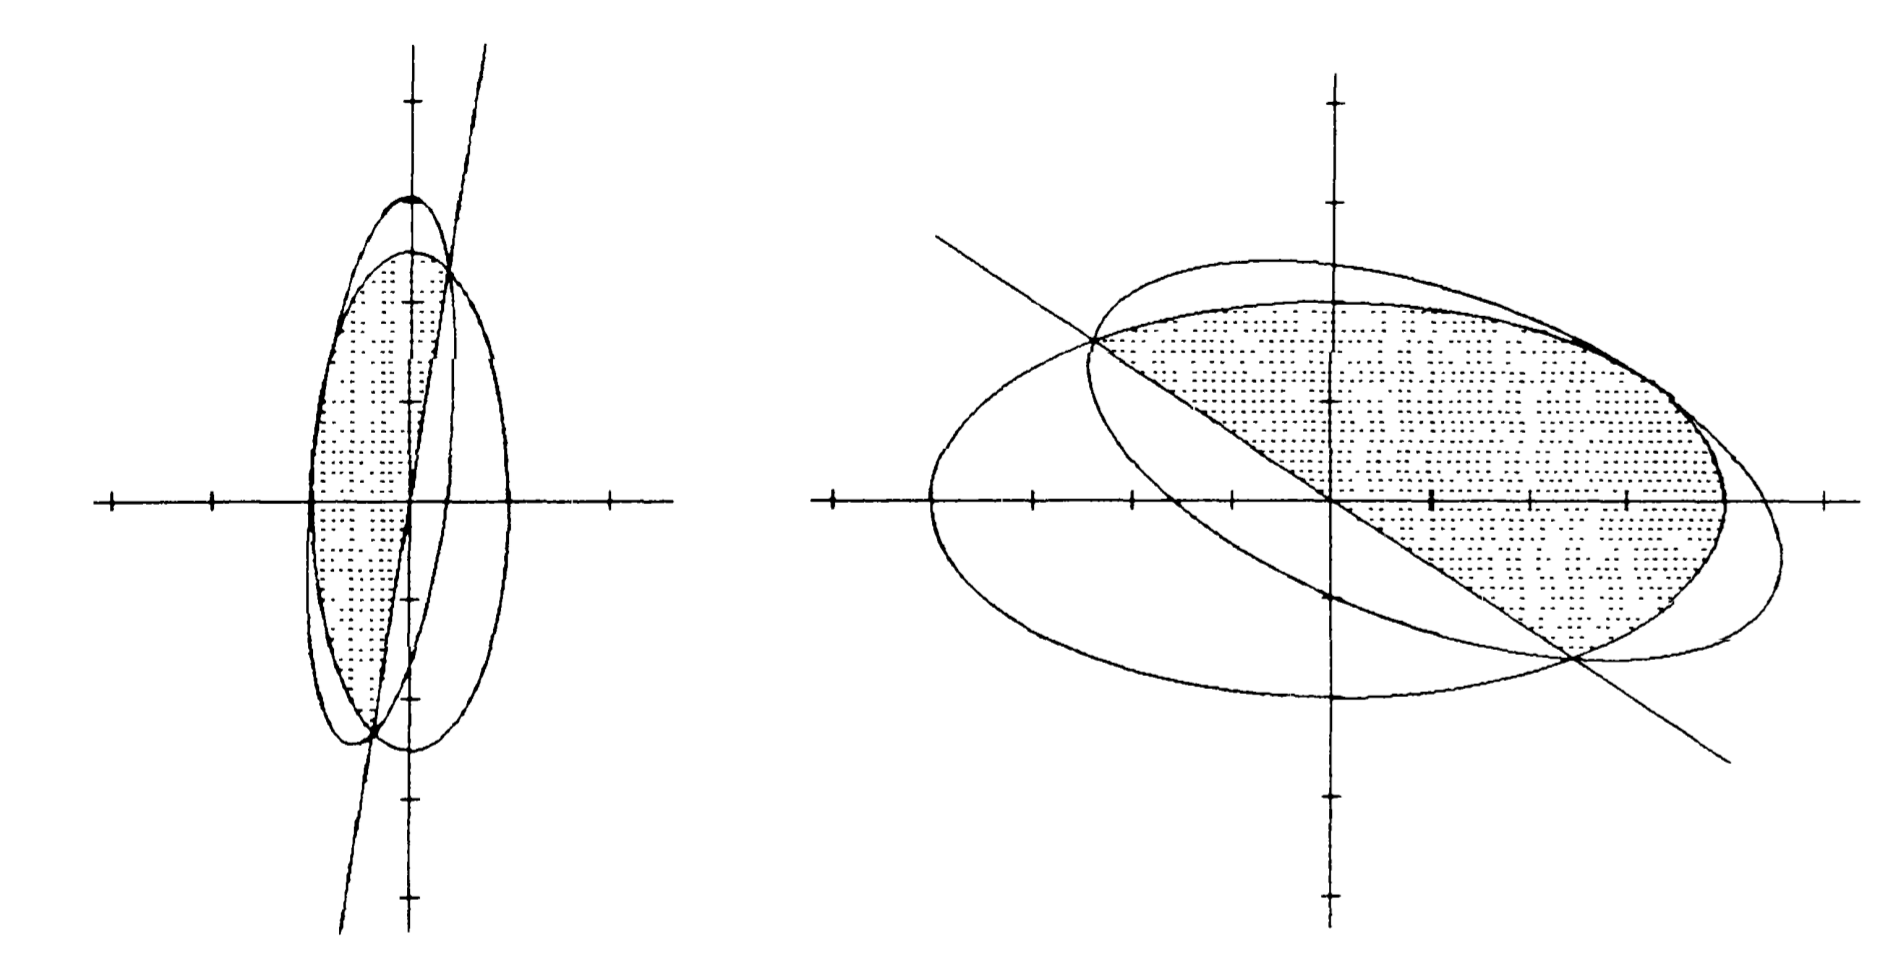
\includegraphics[width=\textwidth]{img/lje}
  \caption{Two ellipsoids and their respective L\"owner John ellipsoids
  corresponding to central cuts. Here the original ellipsoids are cenetered at
  the origin and squared with the \(xy\)-axes.}
  \label{fig:lje}
\end{figure}

After we've made our cut of \(E\), resulting in \(E'\), we want to find the
L\"owner John ellipsoid of \(E'\). In general the L\"owner John ellipsoid of an
arbitrary convex body \(k\) is very difficult to compute, but there are special
cases that can be computed easily; in particular, for the half-ellipsoid
\(E'(A, a, c)\) from the previous section the following offers an explicit
formula for computing the L\"owner John ellipsoid.

\begin{align*}
  b &= \frac{1}{\sqrt{c^T A_k c}} A_k c\\
  a_{k+1} &= a_k - \frac{1}{n+1} b A_k c\\
  A_{k+1} &= \frac{n^2}{n^2-1}\left(A_k - \frac{2}{n+1}bb^T\right)
\end{align*}

Two things to notice:
\begin{enumerate}[(a)]
  \item \(a_{k+1}\) lies on the line from \(a\) to \(z_{min}\)
  \item \(E(A_{k+1}, a_{k+1})\) touches \(E(A,a)\) at \(z_{min}\) and the set 
    \[\partial E(A,a) \cap \{x | c^T x = c^T a\}\]
    This intersection is an ellipsoidal projection into a lower dimension.
\end{enumerate}
